% This is an example on how to use the chalmers-thesis document class.

% Document should be compiled with pdflatex or lualatex
% If you find something odd, wrong or lacking, you can email me at; Mikael Öhman <mikael.ohman@chalmers.se>

% But *please* do NOT email me about standard latex questions, but only things specific to the chalmers-thesis document class.
% I.e. do not ask me about any of the packages included in this example file. Read the manuals for the packages.
% This file has been distributed through: http://www.github.com/Micket/chalmers

% These manuals are a *must* read. They are all full of good examples;
% amsldoc   - http://mirror.ctan.org/macros/latex/required/amslatex/math/amsldoc.pdf
% mathtools - http://mirror.ctan.org/macros/latex/contrib/mh/mathtools.pdf
% biblatex  - http://mirror.ctan.org/macros/latex/contrib/biblatex/doc/biblatex.pdf
% booktabs  - http://mirror.ctan.org/macros/latex/contrib/booktabs/booktabs.pdf
% http://www.ctan.org/tex-archive/help/Catalogue/bytopic.html
% http://en.wikibooks.org/wiki/LaTeX/
% See chalmers-thesis.cls for the documentation on this actual template.

\RequirePackage[l2tabu,orthodox]{nag}
% This package helps prevent you from doing things wrong.

% change masters to bachelors if necessary
\documentclass[bachelors,a4paper]{chalmers-thesis}
\usepackage[table]{xcolor}
% All options are; doctorate, licentiate, masters, bachelors, techreport, projectreport, nocover, draft, g5paper,
% and everything the standard report class support.
\usepackage{ifluatex} % Automatic check for luatex.
%\usepackage[style=ieee]{biblatex}
\ifluatex
 \usepackage{fontspec}
 \defaultfontfeatures{Ligatures=TeX} % To support LaTeX quoting style
\else
 \usepackage[utf8]{inputenc} % File encoding, you should try to stick to utf8.
\fi
\usepackage{microtype} % Magically improves typesetting for pdflatex
\usepackage{subfiles} % Convenient use of subfiles in documents. Using \subfile is optional. See README
\usepackage{hyperref} % Required for in document links and document metadata.
\usepackage[swedish, english]{babel}

% More or less required packages
\usepackage{csquotes} % Needed for biblatex
% Biblatex allows you to choose backend, either the old "bibtex", or the new "biber".

\usepackage[firstinits=true, style=ieee, backend=bibtex]{biblatex}


% Modern bibliography facilities (you may change style to numeric)
\usepackage{mathtools} % All your math related needs
\usepackage{tikz} % Draw figures. Required for cover page
\usepackage{subfig} % Subfloats

% Read the manuals for the respective package to see the usage;
%\usepackage{pdfpages} % For included other pdf files (like articles).
%\usepackage{thmtools} % For theorems.
%\usepackage{algorithms} % For algorithms.
\usepackage{listings} % For source code.
\usepackage{color}  % Custom colors
\usepackage{float}
%\usepackage{booktabs} % High quality tables.
%\usepackage{siunitx} % For all your numerical values and units.
%\usepackage{pgfplots} % Make plots directly in latex. Also tables. Excellent package.
%\usepackage{contmech} % Custom package for typesetting in continuum mechanics for applied mechanics.
%\usepackage{yourcustomcommands} % Put your custom commands in a file 'yourcustomcommands.sty' and load it like this.
\usepackage[toc,page]{appendix}

\usepackage{lipsum}\setlipsumdefault{1-3} % Package used to put in placeholder text. Remove it.

% User commands
\title{Rymd}
\subtitle{Distributed Encrypted Peer-To-Peer Storage} % Optional
\author{Niklas Andréasson \and Robin Andersson \and Johannes Ringmark \and Johan Brook \and Robert Edström}
\thesisin{Computer Science}%%needs to bee changed
\department{Department of Computer Science and Engineering}
\division{Division of Networks and Systems}
\reportno{2014:01}
\copyrightyear{2014}

% Use floats to prevent page breaks in code
\floatstyle{plain} % optionally change the style of the new float
\newfloat{Code}{H}{myc}

% Colors
\definecolor{lightblue}{rgb}{0.21,0.57,0.82}
\definecolor{lightgreen}{rgb}{0.44,0.64,0.19}
\definecolor{lightred}{rgb}{0.84,0.33,0.33}
\definecolor{lightgray}{rgb}{0.4,0.4,0.4}
\definecolor{lightorange}{rgb}{0.71,0.44,0.0}
\definecolor{gray75}{gray}{0.75}

% Fancy chapter titles
\usepackage{fancyhdr} % For page styles
\newcommand{\hsp}{\hspace{20pt}}
\usepackage[T1]{fontenc}
\titleformat{\chapter}[hang]{\Huge\bfseries}{\thechapter\hsp\textcolor{gray75}{|}\hsp}{0pt}{\Huge\bfseries}

% Custom appendix page style
\fancypagestyle{appendix}{%
    \fancyhead{} % Clear all
    \renewcommand{\headrulewidth}{0pt}
}
\setlength{\headheight}{15pt} % fixes \headheight warning

% Increase spacing in non-empty chapters in ToC
\usepackage{etoolbox}
\preto\section{%
  \ifnum\value{section}=0\addtocontents{toc}{\vskip\baselineskip}\fi
}

% Code settings

% Add Javascript language
\lstdefinelanguage{JavaScript}{
  keywords={break, case, catch, continue, debugger, default, delete, do, else, finally, for, function, if, in, instanceof, new, return, switch, try, typeof, var, void, while, with},
  keywordstyle=\color{lightblue}\bfseries,
  ndkeywords={class, export, boolean, throw, implements, import, this},
  ndkeywordstyle=\color{lightred}\bfseries,
  identifierstyle=\color{black},
  sensitive=false,
  comment=[l]{//},
  morecomment=[s]{/*}{*/},
  commentstyle=\color{lightgray}\ttfamily,
  stringstyle=\color{lightgreen}\ttfamily,
  morestring=[b]',
  morestring=[b]"
}

\lstset{
  language=JavaScript,
  extendedchars=true,
  basicstyle=\small\ttfamily,
  columns=fullflexible,
  showstringspaces=false,
  captionpos=b,
  xleftmargin=1.5em,
  xrightmargin=1.5em,
  aboveskip=2\baselineskip,
  belowskip=\baselineskip
}

% Dropping initial letter color
\usepackage{type1cm}
\usepackage{lettrine} % For drop caps
\renewcommand{\LettrineFontHook}{\color[gray]{0.5}}

% You should scale the figure according to textwidth and or paperheight.
% \coverfigure{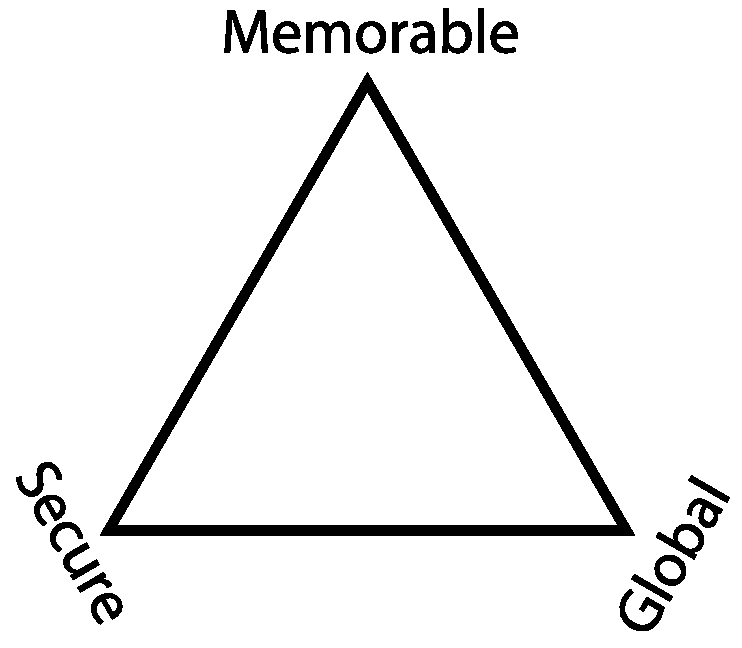
\includegraphics[width=\textwidth,height=0.4\paperheight,keepaspectratio]{figures/Zooko_s_Triangle}}
% \covercaption{Some explanation}

%\renewcommand{\firstabstract}{}

\firstabstract{% Abstract checklist:
%  http://users.ece.cmu.edu/~koopman/essays/abstract.html
%
% Subject
% Motivation
% Problem statement
% Approach
% Results
% Conclusions

This Bachelor's thesis describes the development of a decentralized peer-to-peer file sharing system, bundled as a Javascript developer library. Through evaluations the project determines if it is possible to implement such a system solely with current web technologies. The Namecoin blockchain is used for storing user identities mapped to their public encryption keys, which in turn are used to encrypt data. The end result is a web application where a user can share a file securely with another user completely with peer-to-peer technology.

The final product also includes a front-end prototype is built to show the features of the library. By making the system highly modular (the code split into many separate modules), we manage to achieve satisfying results in reliability and technical agnosticism in terms of underlying implementations.

Even though this project succeeds with its goal of creating a client-side file sharing library, there are still advancements to be made within the area of cryptography for the web.

Computer-aided formalization of mathematics has progressed in the last decade with the formalization of very large and complex proofs such as the proof of the Four color theorem and the Feit-Thompson theorem. In this report we present a formal proof of the Toom-Cook algorithm using the Coq proof assistant together with the SSReflect extension. The Toom-Cook algorithm is used to multiply polynomials and can also be used for integer multiplication.
}
\secondabstract{swedish}{Detta projekt syftar till ta fram ett modulärt bibliotek i JavaScript som är avsett för utvecklare och går under namnet \emph{Rymd}. Biblioteket tillhandahåller säker filöverföring direkt mellan webbläsare. Projektet innefattar utvärdering av moderna webbtekniker för att säkerställa de mest lämpade alternativen.

Drivkraften till projektet kommer från viljan att öka enskilda användares kontroll över sin egen data. Detta i kontrast till dagens trender där externa parter driver centraliserade tjänster för exempelvis chattapplikationer, datalagring och filöverföring. Något som genomsyrar hela projektimplementationen är säkerhet, decentralisering, anonymitet samt modularitet. 

Som demonstration av Rymds funktionalitet skapades även en webbapplikation vid namn \emph{Shuttle}. För datalagring används IndexedDB medan peer-to-peer-kommunikationen utnyttjar WebRTC. Vidare används det ej färdigställda Web Cryptography API för kryptografiska operationer såsom kryptering, dekryptering, signering, med mera. För att lagra kryptografiska nycklar används kryptovalutan Namecoins så kallade \emph{blockchain} där nycklarna är mappade mot användaralias.

Projektet mynnade i slutändan ut i en fungerande fildelningsplattform, med vissa brister i säkerheten. Detta härleds direkt till det tidiga utvecklingsstadiet i de webbteknologier som används. Då webben utvecklas i en rasande takt av både företagen bakom webbläsare samt av standardiseringsorgan är vi däremot säkra att detta rättas till så småningom. Med säker kommunikation direkt mellan klienter kommer anonymitet få ett stort fäste. Vi ser med spänning på vad framtiden har att erbjuda.
}
\keywords{peer-to-peer, distributed, cryptography, file sharing, JavaScript, IndexedDB, WebCrypto, Namecoin}

%\preface{\lipsum} % You can use \input to put preface and acknowledgements in another document
%\acknowledgements{\lipsum}

% You can add extra contents such as abbreviations and nomenclature using.
% Use \presectiontitle to render add titles to new sections.
%\extrafrontmatter{\presectiontitle{Nomenclature} \lipsum} % Optional

% Other optional settings for biblatex;
\DeclareFieldFormat[article]{title}{#1} % Removes quotes from article title
\DeclareFieldFormat[article]{volume}{\mkbibbold{#1}} % Makes volume print in bold.
\renewbibmacro{in:}{} % Removes the "In:" from the journals field.
\DeclareFieldFormat[article]{pages}{#1} % Removes the pp. before pages.
% Adds short journal entries;
\renewbibmacro*{journal+issuetitle}{%
  \usebibmacro{shortjournal}%
  \setunit*{\addspace}%
  \iffieldundef{series}{}{\newunit\printfield{series}\setunit{\addspace}}%
  \usebibmacro{volume+number+eid}%
  \setunit{\addspace}%
  \usebibmacro{issue+date}%
  \setunit{\addcolon\space}%
  \usebibmacro{issue}%
  \newunit}
% End of optional citation modifications.

\addbibresource{References.bib} % New command, use if available
%\bibliography{References} % Legacy command

\begin{document}


%\selectlanguage{swedish} % Use this if you are writing your thesis in swedish.
%\makecoverpage
%\maketitle
% If you need to do any modifications, you can redefine each page respectively, or just call them manually as;
 \setcounter{page}{-100} % Necessary to give the first pages a unique identifier using hyperref.
   \makecoverpage

  \maketitlepage

  \makeprintinfopage

 \newpage
 \pagenumbering{roman}
 
 % Increase page margins for abstract pages
 \newgeometry{left=0.22\paperwidth, right=0.22\paperwidth}
    \makeabstractpage\pagestyle{plain}
    \makesecondabstractpage
  \restoregeometry

  %\makeacknowledgementspage


  \cleardoublepage

  \presectiontitle{Terminology}
  \section*{General terminology}
\begin{description}
  \item[Adobe PhoneGap] A software enabling development of cross-platform hybrid smartphone applications - applications developed using web technologies, but packaged as native smartphone binaries.
  \item[API] Application Programming Interface. An interface that software developers can use to get easy access to data and/or particular functionality for their software. Typically exposed as a software library or HTTP service.
  \item[Bitcoin] The first and biggest widespread cryptocurrency.
  \item[CA] Certificate Authority. A third party that is trusted to verify the validity of public keys and certificates.
  \item[Chrome Apps] Similar to Adobe PhoneGap, but for desktop applications running in a Google Chrome sandbox.
  \item[Cloud storage] A service that hosts data externally with seamless access over the internet.
  \item[Cryptocurrency] A network transaction system that uses a fully distributed cryptographically secured ledger (called the \emph{blockchain}) to track transactions. The vast majority of cryptocurrencies are forks off Bitcoin.
  \item[Centralized system] A system which has several nodes connecting and depends on one or a few central endpoints.
  \item[Decentralized] A system where responsibilities are shared across the nodes and does not depend on a single, central endpoint.
  \item[DHT] Distributed Hash Table. A notion in computer science of a distributed key-value store.
  \item[Firefox OS] A smartphone operating system where all applications are web-based.
  \item[GUID] Globally Unique Identifier. Used as pseudo-unique identifiers, such as keys in a database. Usually 128-bit values stored as 32 hexadecimal in groups separated by hyphens.
  \item[NoSQL] All database systems which are not modelled in tabular relations. Examples are graphs, trees, and key-value stores.
  \item[OpenPGP] A standard for data encryption and signing, originally coming from the proprietary software Pretty Good Privacy (PGP) and widely spread through the free implementation GPG.
  \item[P2P] Peer-to-peer. Distributed, direct communication.
  \item[PKI] Public Key Infrastructure.A system that associates (unique) user identities with their public keys. Typically implemented as a Web of Trust or with one or several CAs. Typically, trusted parties use their private keys to sign the public keys of users to verify the connection between an identity and a public key.
  \item[RSA] A widely used public-key cryptosystem. As such, it builds on pairs of private and public keys where encryption with one can be reversed with decryption of the other. This system is asymmetric and the security relies on the practical difficulty of factoring the product of two large prime numbers.
  \item[PKI] Public Key Infrastructure. A system that associates (unique) user identities with their public keys. Typically implemented as a Web of Trust or with one or several CAs. Typically, trusted parties use their private keys to sign the public keys of users to verify the connection between an identity and a public key.
  \item[RDBMS] Relational Database Management System, a popular type of database management system based on the relational model.
  \item[SQL] Structured Query Language, is a language for managing, querying and manipulating data in relational database systems.
  \item[SQL injection] A technique for injecting malicious SQL code into the executing database queries in order to, for instance, dump the contents of the database.
  \item[XSS] Cross Site Scripting is the technique for injecting client side scripts into web pages on other domains.
  \item[Web of Trust] A type of distributed PKI that builds on peer-to-peer trust. If Alice trusts Bob, then Bob is trusted introduce new identities and public keys for Alice.
\end{description}

\section*{Terms with specific meaning in the Rymd project}
\begin{description}
  \item[Identity] A unique, memorable string identifying a user within the network.
  \item[Module] A delimited area of interest and functionality in system architecture.
  \item[Node] A client in the network (such as a web browser).
  \item[Resource] A file or folder in the network (a thing that can be shared between nodes)
  \item[Rymd] The developer library for web based peer-to-peer sharing – the main product. Is also the Swedish word for \emph{space}, which encompass the main ideas of the project.
  \item[Shuttle] A web based file sharing application implemented using Rymd to demonstrate the basic capabilities of the project.
\end{description}


  \cleardoublepage
 \tableofcontents

 % Sets up page numbering for the rest of the document.
  \cleardoublepage
 \pagenumbering{arabic}
%\makeprintinfopage
%\makededicationpage
%\makeprefacepage
%\makeacknowledgementspage
% \maketableofpaperspage

% Main layout
\subfile{Layout}




\end{document}
